\thispagestyle{empty}


Digital infrastructures are the backbone of our societies, as we can
observe in times of a crisis: teleworking, telemedecine, distance
learning, etc. are the basis of our resilience.
In such situations, as well as in more common ones, the solidity of
our societies depends on the reliability of these infrastructure: a
single bug can cause people to die and enterprises to go bankrupt.

If testing software makes it possible to reveal the the presence of
bugs, only formal verification can guarantee their absence.  Thus, the
trust in critical systems relies on formal verification, in particular
computerised formal proofs, that guarantee the safety of people using
transportation systems (autonomous cars, subways, trains, planes,
etc.), health systems (robotic surgery, ear implants, telemedecine,
etc.), energy provided by nuclear plants, financial applications,
e-governance, etc.

This crucial role of computerised formal proof is highlighted by
several successes, like the correctness proofs of the automatic Paris
metro line 14 \cite{Behm98,Lecomte17}, the detect-and-avoid system for
unmanned aircraft system developed by NASA \cite{Munoz16}, the
operating system seL4 \cite{Klein09}, or the C compiler CompCert
\cite{Leroy06}.  It has been empirically observed that operating
systems and compilers often have bugs, but proved systems and
compilers, such as seL4 or CompCert, have none, or much fewer.  This
is why, at the highest Evaluation Assurance Levels (EAL) of the Common
Criteria (CC) security evaluation international standard, in effect
since 1999, certification processes require proofs, and not only
testing.

% TODO: Should we give specific examples here already?
Several companies in our consortium from sectors such as
transportation, health case, and energy have expressed interest in
using formal methods or scaling up their existing use of them. These
companies are at the forefront of the adaptation of formal methods in
the industry, and if they are successful many others will likely
follow. By making formal methods more accessible to these companies
and all other interested partners, via better theories, better tools
and better-training of workers, we hope bring a significant
competitive advantage to European companies and Europe as a whole.

Aside from their use in software verification, proofs have also always
been the basis of mathematics, and hence of many mathematised
sciences. In this area, the use of computerised formal proofs has made
significant progress, as witnessed by the formalisation of the
Feit-Thompson theorem \cite{Gonthier13}.  Such a use of formal proofs
in mathematics and in sciences is important, as the correctness of a
pencil and paper proof is often the object of a controversy, as shown
by the case of Hales' theorem (Kepler's conjecture) which is too long
and too complex to be verified without a computer (and which has now
been formally verified \cite{Hales17}) or with the more recent
controversy on the $abc$ conjecture {\color{red} reference}. Thus,
formal proofs have a wide range of applications, from safety and
security of software to mathematics.

Formal proofs are developed using research infrastructures called
``proof systems''.  These proof systems are pieces of software that
allow computer scientists, mathematicians, engineers, and logicians to
build and study formal proofs, just like particle accelerators allow
physicists to build and study particles. Figure \ref{systems} lists
the most prominent proof systems today.

%%%%%%%%%%%%%%%%%%%%%%%%%%%%%%%%%%%%%%%%%%%%%%%%%%%%%%%%%%%%%%%%%%%%%%%%%%%%%%
\newcommand\s{ $\star$}
\begin{figure}[ht]
  \definecolor{shadecolor}{named}{color1}
  \begin{shaded}
    \begin{center}
      {\bf \Large Major proof systems}\\[5mm]
      \begin{tabular}{|c|c|}\hline
       {\bf In Europe} & {\bf Outside Europe}\\\hline
        \begin{minipage}{10cm}
          \begin{tabular}{cccc}
            Abella & Agda\s & Atelier B\s & Coq\s\\
            FoCaliZe\s & HOL4\s & Isabelle\s & KProver\s\\
            Matita\s & Minlog\s & Mizar\s & ProB\\
            ProvenTools\s & Rodin\s & \tlaplus\s & Why3\s\\
          \end{tabular}
        \end{minipage}
        &\begin{minipage}{4cm}
           \begin{tabular}{cc}
             Acl2 & HOL Light\s\\
             IMPS & Lean\\
             LFSC\s & NuPRL\\
             PVS\s & TSTP\s
           \end{tabular}
         \end{minipage}\\\hline
      \end{tabular}
    \end{center}
    \vspace{-5mm}
    \caption{Those addressed in the project are marked with $\star$.\label{systems}}
  \end{shaded}
\end{figure}

%%%%%%%%%%%%%%%%%%%%%%%%%%%%%%%%%%%%%%%%%%%%%%%%%%%%%%%%%%%%%%%%%%%%%%%%%%%%%%

A lot of formal proofs developed for one critical system could be used
in another.  Unfortunately, the development of formal methods is
slowed down by the large number of proof systems (and sometimes the
large number of versions, over time, of one single system) and the
lack of a common theory used by these systems.  For instance, the
Paris metro line 14 has been proved correct in Atelier B, while the
NASA detect-and-avoid system for unmanned aircraft system has been
proved correct in PVS, the seL4 operating system has been proved
correct in Isabelle/HOL\cite{paulson700}, and the compiler CompCert
has been proved correct in Coq.  Some projects, such as the proof of
Hales' theorem, have been started in different systems and required
significant integration efforts for obtaining the overall result.

Because of the focus on this large variety of proof systems, the field
is fragmented into a number of small communities, each of which is
centered around one theory and one proof system. This proposal brings
together partners from a large number of these different communities
for the first time, and brings them together in a new community
centered around the development of a shared infrastructure for formal
proofs. In fact, the initial interest for this proposal was so big
that the number of participants had to be limited.  This clearly
demonstrates the potential for this new community to grow further
during and after the course of this project.

The fragmented nature of the current proof systems is a major
bottleneck for the adaptation of formal systems by the
industry. Several of the companies in our consortium have expressed
interest in the use of formal methods, but are faced with the
difficult task of choosing a proof system to work with. In general, a
library developed in one system cannot be used in another, so a wrong
choice may lead to a critical library being unavailable in that
system. This forces the company to either develop the library
themselves or switch to a different proof system.  Thus,
interoperability (the possibility for one user to use a proof
developed in another system), sustainability (the possibility to use a
proof decades after it has been developed), and cross-verification
(the possibility to verify a proof in a system different from the ones
in which it has been constructed resulting in a higher assurance of
its correctness) are restricted.

The fragmentation of these infrastructures also limits the
dissemination of formal proofs in non-specialist communities. For
instance, teaching formal proving to undergraduate students in a logic
course is difficult, as it requires the choice of a specific language,
a specific theory, and a specific system that restrict the scope of the
course, instead of giving students the tools that are useful
everywhere. 

An important goal of this project is thus to provide free and virtual
access to these critical libraries from all proof systems,
which will greatly increase the adoption of formal verification in
both industry and education.

% Jesper: I don't think this paragraph adds much to the main story here.
%On philosophical grounds, while we had in the past an (informal) proof
%of Pythagoras' theorem or Fermat's little theorem, the same proof now
%has different formalizations in PVS, Isabelle/HOL, Coq, etc.  Thus,
%the universality of logical truth itself has been threatened. 
%As we shall
%see, it is not the first time in history that this universality of
%logical truth is jeopardized: it already has been, for instance, in
%the 19$^{\mbox{\footnotesize th}}$ century, with the non-Euclidean
%geometries. This crisis of the non-Euclidean geometries has been
%solved at the beginning of the 20$^{\mbox{\footnotesize th}}$ with the
%invention of a logical framework: predicate logic
%\cite{HilbertAckermann}, in which the various geometries could be
%defined.

%%%%%%%%%%%%%%%%%%%%%%%%%%%%%%%%%%%%%%%%%%%%%%%%%%%%%%%%%%%%%%%%%%%%%%%%%%%%%%
\begin{center}
$\bigstar$ $\bigstar$ $\bigstar$
\end{center}

Making proof systems interoperable would avoid duplication of work,
reduce development time, enable cross-verification, and make formal
proofs accessible to a much larger community.  

After three decades
dedicated to the development of these systems, allowing such a
cooperation between systems is the next step in the development of the
formal proof technology.

\medskip

\hspace{-0.8cm}
\begin{tabular}{p{0.4\textwidth}p{0.6\textwidth}}
\begin{minipage}{7cm}

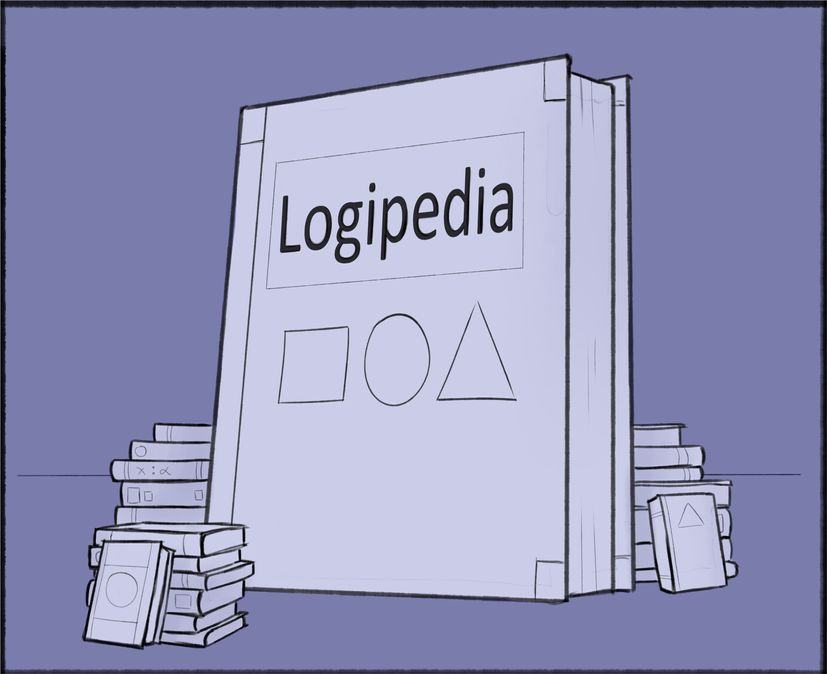
\includegraphics[width=7cm]{img/Illustration3-reduced.jpg}

{\em \small Artwork by Nadia Miller.}

\end{minipage}
&
\begin{minipage}{9.85cm}

To bring together the fragmented field of formal methods and to
provide everyone -- no matter what proof system they use -- with free
and open access to libraries of formal proofs, we propose to develop
an encyclopedia that will eventually contain all formal proofs in
existence.

\begin{center} \textbf{This encyclopedia will be called Logipedia.} \end{center}

Building such an encyclopedia will allow interoperability,
sustainability, and cross-verification of all formal proofs in the
encyclopedia.
  
\end{minipage}
\\
\end{tabular}

\medskip

%\hspace{0.4cm} Each proof system comes with its own libraries, and
%these libraries are also part of research infrastructures. To address
%the challenge of improving cooperation between these proof systems, we
%will integrate these libraries in an online encyclopedia of formal
%proofs. Each proof in this encyclopedia will have versions in each
%theory where it can be expressed, so that it can be used in as many
%systems as possible.  

%\hspace{0.4cm} As each proof system implements a different theory,
%Logipedia will contain proofs expressed in different theories.  Such a
%theory-independent infrastructure is possible, because the
%theories implemented in these different proof systems can be expressed
%in a common logical framework: the $\lambda \Pi$-calculus modulo
%theory, implemented in the system
%\href{https://deducteam.github.io/}{Dedukti}. Dedukti is thus the {\em
%  lingua franca} that permits this theory-independent encyclopedia to
%exist.


Logipedia is thus a research infrastructure that integrates proof
systems, through the sharing of data (formal proofs).

\begin{itemize}
\item Logipedia will bring together the communities centered around
  different proof systems, providing new opportunities for networking
  between these previously separate communities.

\item Logipedia will provide a vast library of proofs developed in
  different proof systems and make them available to the public,
  greatly increasing the trans-national and virtual access to these
  valuable resources.

\item Logipedia will allow researchers from different areas to share
  and discuss their work in a common language, opening up new avenues
  for joint research activities.
\end{itemize}


%%%%%%%%%%%%%%%%%%%%%%%%%%%%%%%%%%%%%%%%%%%%%%%%%%%%%%%%%%%%%%%%%%%%%%%%%%%%%%
\begin{center}
$\bigstar$ $\bigstar$ $\bigstar$
\end{center}

\begin{tabular}{p{0.7\textwidth}p{0.3\textwidth}}
\begin{minipage}{11.85cm}
\hspace{0.4cm} Such an infrastructure is, in many ways, new in the
European Strategy on Research Infrastructures. In fact, the idea to
structure a networking activity around the construction and the use of
a large scale infrastructure is itself relatively new in computer
science and mathematics, even though some efforts have been made in
this direction with the {\em OpenDreamKit} and {\em Software
  Heritage}, for example.

\hspace{0.4cm} So, we also aim at contributing to an evolution of the
organisation of research in the computer science and mathematics in
Europe.
\end{minipage}
&
\begin{minipage}{4cm}

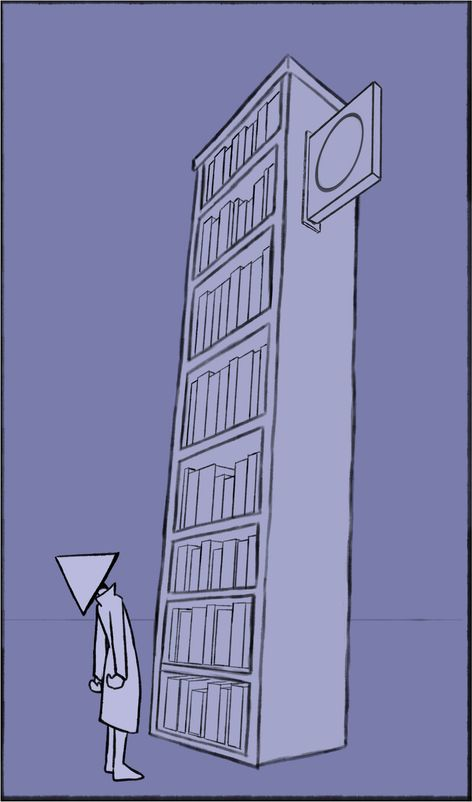
\includegraphics[width=4cm]{img/Illustration1-reduced.jpg}

\end{minipage}
\\
\end{tabular}



\begin{center}
\end{center}



%%%%%%%%%%%%%%%%%%%%%%%%%%%%%%%%%%%%%%%%%%%%%%%%%%%%%%%%%%%%%%%%%%%%%%%%%%%%%%
\definecolor{shadecolor}{named}{color2}
\begin{shaded}
  \vspace*{-0.5cm}
  \begin{center}
    {\bf \Large History of the project}
  \end{center}

Convinced that a cloud of formal proofs could bring to the
applications of formal proof technology the same boost that the cloud
has brought to computing, and also that managing a large encyclopedia
required some interdisciplinary effort,
we developed a proof of concept containing a few hundreds lemmas
expressed in the language of six systems and organized, in January 2019,
a meeting to discuss the future of this project.
This
meeting brought together 38 researchers from Austria, the Czech
Republic, France, Italy, the Netherlands, and Poland.
\begin{center}
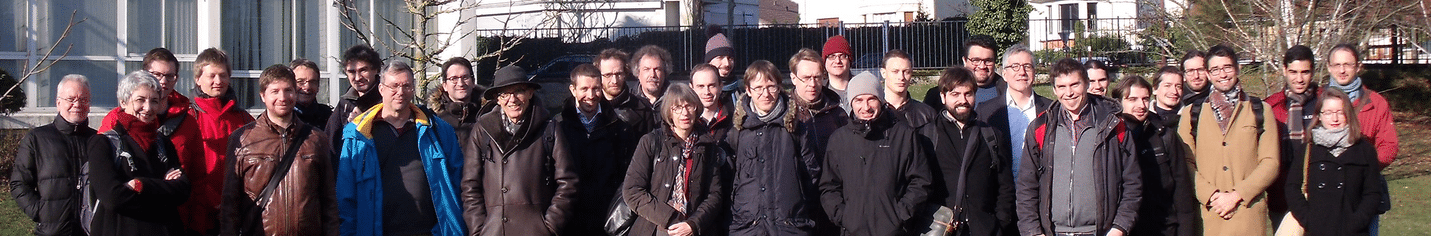
\includegraphics[height=2cm]{img/Photo-reduced.png}
\end{center}
During this meeting, the idea of making this proof of concept a
European infrastructure emerged.  Since then, colleagues from Belgium,
Germany, Romania, Serbia, Sweden, and the United Kingdom, from
academia and industry, have expressed their interest in participating
in this effort.  These researchers and engineers are ready to
contribute to develop this encyclopedia, aiming at sharing proofs,
under a creative commons licence, making them searchable, accessible,
interoperable, and reusable.
\end{shaded}


%%%%%%%%%%%%%%%%%%%%%%%%%%%%%%%%%%%%%%%%%%%%%%%%%%%%%%%%%%%%%%%%%%%%%%%%%%%%%%
\begin{framed}
\vspace*{-0.5cm}
\begin{center}
{\bf \Large How do proofs contribute to safety and security of software?}
\end{center}

Imagine the following casino game. At the beginning, a player is given
eleven euros. At each round, she throws a six-sided dice. If the
result is a six, then the game ends.  If it is a five, a four, a
three, or a two, she is given twice the amount of money she already
has. If it is a one she loses two euros, if she has at least two.
When the game ends, the player wins the money she got, except if she
has zero, in which case she loses one million euros.

This game can be modeled by the following programme:
\begin{center}
\begin{minipage}{10cm}
\begin{verbatim}
n = 11
stay = True;
while stay:
    roll = random.randint(1,6)
    if roll == 6:
        stay = False
    else:
        if roll >= 2:
            n = n + 2 * n
        else:
            if (n >= 2):
                n = n - 2
print(n)
\end{verbatim}
\end{minipage}
\end{center}

To be on the safe side, the player wants to be sure, before starting
playing, that she will never finish with zero.  And indeed, at all times
the content of the variable {\tt n} is an odd number,
thus it cannot be zero. {\bf This property ``nothing bad happens'' is
called the ``safety'' of this program.} This property is a
consequence of two simple theorems of arithmetic:
$$\forall x~(\mbox{\it odd}(x) \Rightarrow \mbox{\it odd}(x + 2 * x))$$
$$\forall x~(\mbox{\it odd}(x) \Rightarrow \mbox{\it odd}(x - 2))$$
meaning that, for all $x$, if $x$ is an odd number, then $x+2*x$ and $x-2$ are odd numbers too.
Hence, proving the safety of this programme amounts to prove these two
theorems.

Let's now consider the case where there is a tiny bug in the
programme. For instance the {\tt 2} has been replaced by a {\tt 3} in
the instruction {\tt n = n + 2 * n}. The programme is then unsafe as
shown by the sequence $11, 9, 7, 5, 3, 1, 4, 2, 0$. Yet, testing this
program will, most likely, not reveal this bug, since it only
manifests very rarely.  In contrast, attempting to prove the
correctness of this program will reveal the bug as it is impossible to
prove the proposition
$$\forall x~(\mbox{\it odd}(x) \Rightarrow \mbox{\it odd}(x + 3 * x))$$
\end{framed}

%%%%%%%%%%%%%%%%%%%%%%%%%%%%%%%%%%%%%%%%%%%%%%%%%%%%%%%%%%%%%%%%%%%%%%%%%%%%%%
%\begin{shaded}
%\vspace*{-0.5cm}
%\begin{center} {\bf \Large When mathematics are needed to verify the
%    correctness of a programme}
%\end{center}
%
%Prime numbers are used in a wide variety of applications:
%pseudo-random number generation, cryptographic algorithms, etc.  Thus,
%verifying the correctness of complex primality testing algorithms is
%critical.
%
%To do so, we need first to define primality, for instance
%
%$$prime(p) := 1<p \wedge (\forall n, (1<n\wedge n<p) \Rightarrow \neg(n\mid p))$$
%
%where $\wedge$ is the conjunction, $\Rightarrow$ is the implication,
%$\neg$ is the negation, and $n\mid p$ means that $n$ divides $p$.
%
%To lower the cost of primality testing, we use tests that are more
%efficient than the naive use of the definition.  For instance, a very
%simple improvement is to test the divisibility of the considered
%number, not by each of the smaller natural numbers, but only up to its
%square root.  Indeed, if a natural number $p$ can be factored into the
%product of two smaller natural numbers $m$ and $n$, one of them has to
%be smaller than or equal to the square root of $p$.  Therefore, one
%could give the following more complex, but more efficient, definition:
%
%$$prime'(p) := 1<p \wedge (\forall n, (1<n \wedge n*n\leq p) \Rightarrow \neg(n\mid p))$$
%
%To ensure that these definitions are equivalent one needs to prove
%the following statement:
%
%$$\forall p, prime'(p) \Leftrightarrow prime(p)$$
%
%It would have been easy to introduce a small bug
%in the new definition.  For example, one could have written
%$n*n < p$, instead of $n*n \leq p$.
%This would have resulted in accepting squares of primes as primes.
%
%Yet, attempting to prove the equivalence of these two definitions would
%have revealed the bug, as they cannot be proven to be equivalent.
%\end{shaded}

%%%%%%%%%%%%%%%%%%%%%%%%%%%%%%%%%%%%%%%%%%%%%%%%%%%%%%%%%%%%%%%%%%%%%%%%%%%%%%
\begin{framed}
  \vspace*{-0.5cm}
  \begin{center}
    {\bf \Large What is a formal proof? What is a proof system?}
    \end{center}

Since Antiquity, we have known that
proofs, both purely mathematical ones, as in Euclid's elements or the
recent proof of the Kepler's conjecture by Thomas Hales, and proofs used
to establish the safety and security of software, can be built with a
limited number of rules, for example
\begin{itemize}
\item From $A\Rightarrow B$ (``$A$ implies $B$'') and $A$, deduce $B$.
\item From $A$, deduce $A\vee B$ (``$A$ or $B$'').
\item etc.
\end{itemize}
Yet for most of mathematical history, proofs have been written in
a pidgin of natural language and mathematical formulas. When proofs are
very long (as it is often the case for the proofs used in safety and security,
but also for some proofs in pure mathematics), mistakes are
very difficult to detect. For instance, dozens of wrong proofs of
the parallel postulate have been given through history, sometimes by the
best of mathematicians such as Ptolemy, Proclus, al-Haytam, Tacket,
Clairaut, Legendre, etc.

In the 1960s, Robin Milner and Nicolaas de Bruijn noticed that the
correctness of a mathematical proof could be checked by a
computer. This led to the development of the two first proof systems
in history: Milner's LCF and de Bruijn's Automath.

For instance, from the axioms
$$\forall x~(\mbox{\em philosopher}(x) \Rightarrow \mbox{\em human}(x))$$
$$\forall x~(\mbox{\em human}(x) \Rightarrow \mbox{\em mortal}(x))$$
we can deduce
$$\forall x~(\mbox{\em philosopher}(x) \Rightarrow \mbox{\em mortal}(x))$$
In the language implemented in Automath, this proof is written
$$\lambda x \lambda h~(g~x~(f~x~h))$$
\end{framed}

%%%%%%%%%%%%%%%%%%%%%%%%%%%%%%%%%%%%%%%%%%%%%%%%%%%%%%%%%%%%%%%%%%%%%%%%%%%%%%
\begin{framed}
\vspace*{-0.5cm}
  \begin{center}
{\bf \Large What is a theory?}
\end{center}

Deduction rules such as ``From $A \Rightarrow B$ and $A$, conclude
$B$'' are universal, but building proofs requires more rules, that are
often specific to a domain of knowledge and are called
``axioms''. Examples are the axioms of geometry, the axioms of
arithmetic, etc. These axioms constitute a theory.

At the beginning of the 20$^{\mbox{\footnotesize th}}$ century, an
axiomatic theory, {\em set theory}, has been proposed to express all
mathematical proofs. In the first half of the 20$^{\mbox{\footnotesize
    th}}$ century a few variants of set theory have been proposed, as
well as a few alternatives (such as \emph{Simple Type Theory}).  But
because these theories had not been designed for being implemented on
a computer, each proof system such as Coq, Isabelle/HOL, Mizar,
Atelier B, etc. has implemented its own theory.  {\bf Thus, the rise of
computer-checked formal proofs has led to a multiplication of
alternative theories for mathematics.

This is the major obstacle to interoperability between proof systems.}
\end{framed}



%%% Local Variables:
%%%   mode: latex
%%%   mode: flyspell
%%%   ispell-local-dictionary: "english"
%%% End:
